\section{Konzeptionelle Gestaltung des Loggings}

Als Ausgabeformat des Loggings werden Log-Dateien verwendet, um sicherzustellen, dass keine wichtigen Informationen verloren gehen. Log-Dateien bieten zudem die einfache 
Möglichkeit, Methoden wie die Log-Rotation zu implementieren. Die Erstellung einer Datenbank für das Logging des Testprogramms wäre unverhältnismäßig aufwendig und daher nicht 
praktikabel.

Bezüglich der Sicherheit und des Datenschutzes sind keine besonderen Maßnahmen erforderlich, da die Log-Dateien nur lokal gespeichert werden, keine personenbezogenen Daten enthalten 
und nur autorisierte Benutzer Zugriff auf die Log-Dateien haben.

Um die Log-Nachrichten sinnvoll zu kategorisieren, werden verschiedene Log-Level eingeführt. Es wird jedoch auf drei verschiedene Log-Level begrenzt, da dies eine ausreichende 
Abgrenzung der Nachrichten des Testprogramms ermöglicht und die Komplexität für den Benutzer reduziert. Die Log-Level sind wie folgt definiert:

\begin{itemize}
    \item \textbf{Error} (Fehler): Das höchste Log-Level weist auf Fehlerzustände oder Probleme hin, die die ordnungsgemäße Funktion beeinträchtigen. Im Testprogramm kann dies beispielsweise der Fall sein, wenn Bilder oder Bildstapel während der Kommunikation verloren gehen oder die Kommunikation abbricht.
    \item \textbf{Warning} (Warnung): Dieses Level zeigt an, dass etwas Unerwartetes passiert ist, das einen der Prozesse stören kann, aber nicht unbedingt zu einem Funktionsausfall führt. Ein Beispiel hierfür ist eine unerwartete Veränderung der Anzahl der pro Sekunde empfangenen Bilder.
    \item \textbf{Info} (Information): Auf diesem Level werden Informationen des normalen Betriebs dokumentiert, wie das Empfangen der einzelnen Bilder bzw. Bildstapel sowie die Darstellung von Statistiken.
\end{itemize}

Die Formatierung der Log-Nachrichten basiert auf folgendem Muster: 
\vspace*{-15pt}
\begin{center}
  [Zeitstempel] [Log-Level] [Nachricht/Beschreibung]
\end{center}
\vspace*{-15pt}

Damit wird sichergestellt, dass der Zeitpunkt und die Reihenfolge der Log-Nachrichten nachvollziehbar sind. Zudem ist das entsprechende Log-Level direkt sichtbar und eine 
eindeutige Beschreibung der Nachricht vorhanden. Abbildung \ref{fig:Logfile} zeigt beispielhaft den Aufbau der Log-Dateien:

\begin{figure}[htbp]
    \centering
      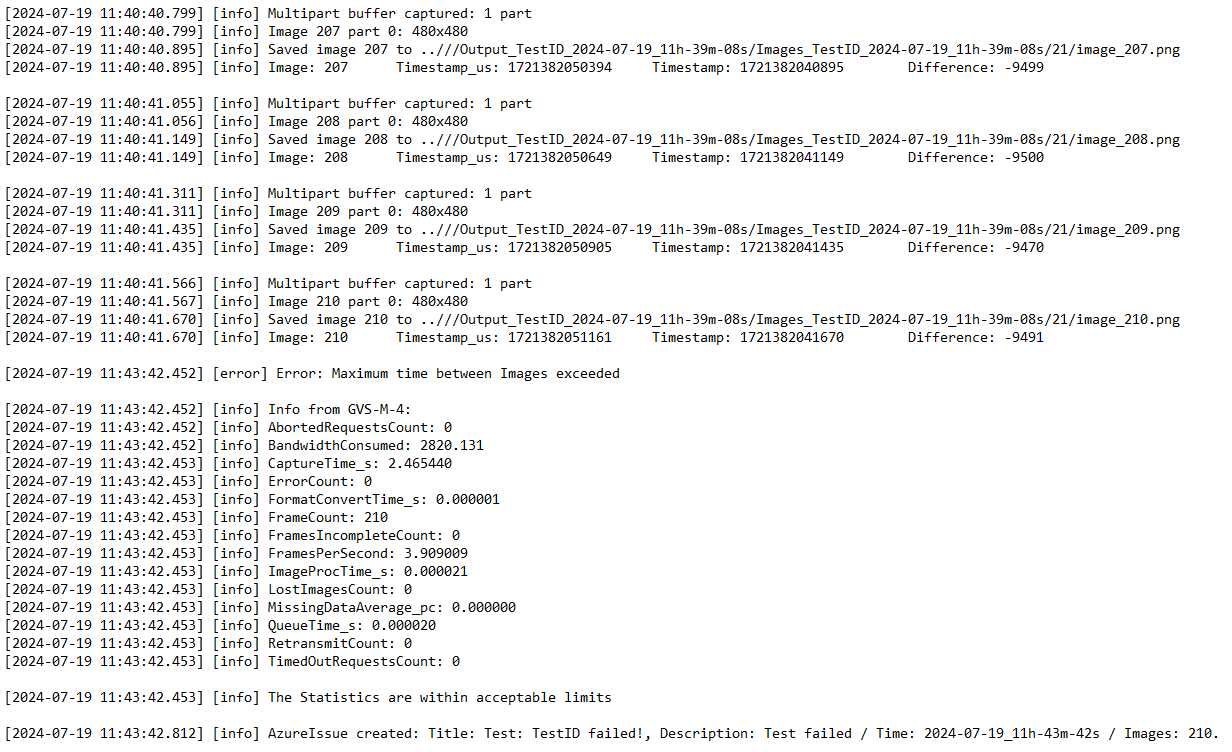
\includegraphics [width=0.9\textwidth]{Logfile.png}
    \caption[Beispiel Log-Datei]{Beispiel Log-Datei (eigene Darstellung)}
    \label{fig:Logfile}
\end{figure}

Um die Performance des Systems nicht zu beeinträchtigen und das Handling der Log-Dateien zu vereinfachen, wird eine Log-Rotation implementiert. Hierbei werden Parameter für die 
maximale Größe einer Log-Datei und die maximale Anzahl an Log-Dateien festgelegt. Der Benutzer kann damit individuell einstellen, wie weit die Informationen der Log-Dateien 
zurückgehen sollen. Eine Archivierung älterer Log-Dateien wird nicht umgesetzt, da der Benutzer bei Bedarf eine entsprechend hohe Anzahl an maximalen Log-Dateien einstellen kann.

Es wird synchrones Logging eingesetzt, da auf die korrekte Reihenfolge und die Vollständigkeit der Logs großer Wert gelegt wird. Zudem ist die Performance des 
Testprogramms nicht in einem solchen Grad entscheidend, dass eine andere Lösung notwendig ist. Durch synchrones Logging bleibt der Quellcode des Testprogramms einfach lesbar und 
es ist nachvollziehbar, an welcher Stelle die jeweilige Log-Nachricht entsteht.

Bei bestimmten Fehlern oder dem erzwungenen Abbruch des Testprogramms wird ein \glqq Azure Issue\grqq\ erstellt, um den Benutzer über das Ereignis zu informieren. Dies ist notwendig, da der 
Benutzer nicht ständig am Testaufbau anwesend ist und Langzeittests auch außerhalb der Arbeitszeit laufen. Diese Funktion arbeitet unabhängig von der Erstellung der Log-Dateien, um 
verzichtbare Abhängigkeiten zu vermeiden.

Um eine klare Trennung der Informationen des Testdurchlaufs von denen des Testprogramms sicherzustellen, werden die Informationen und gegebenenfalls Fehlermeldungen des Testprogramms 
im Terminal ausgegeben. Dies ist sinnvoll, da das Testprogramm direkt nach dem Start die meisten Funktionen durchläuft und anschließend hauptsächlich sich wiederholende 
Abschnitte ausführt. Der Benutzer ist beim Start des Tests in der Regel am Aufbau anwesend und kann daher falls notwendig eingreifen. Für den Fall, dass der Benutzer nicht 
anwesend ist und um die Informationen zusätzlich konsistent zu speichern, wird neben den Log-Dateien für die Datenverarbeitung eine zusätzliche Log-Datei speziell für die 
Überwachung der Funktionen des Testprogramms erstellt. Diese Log-Datei verwendet dieselbe Formatierung wie die anderen Log-Dateien, ist jedoch eine einfache, nicht konfigurierbare 
Datei mit einem festgelegten Log-Level. Dies ist ausreichend, da das Testprogramm nur einen abschätzbaren, begrenzten Umfang an Log-Nachrichten liefert. Außerdem wird dadurch 
vermieden, dass es bei der Konfiguration des Tests durch zu viele Parameter zu Verwirrungen kommt.

Für die Implementierung des Loggings in C++ wird die Bibliothek \glqq spdlog\grqq\ verwendet. Diese ermöglicht eine einfache Konfiguration inklusive des Log-Levels, 
der Formatierung der Log-Nachrichten und der Log-Rotation. Die manuelle Implementierung dieser Eigenschaften über standardmäßige Dateioperationen ist sehr aufwendig und schränkt 
die Flexibilität bei der Konfiguration der Features (z.B. der Log-Rotation) ein. Die Bibliothek \glqq spdlog\grqq\ wird verwendet, da sie eine umfassende Dokumentation 
bietet, benutzerfreundlich ist und viele Konfigurationsmöglichkeiten erlaubt.